\graphicspath{ {../body/nash_bargaining_figures/} }
\chapter{基于议价博弈的多用户资源分配}
\echapter{Bargaining Game on Resource Allocation for Multiple Users}
%\label{chap_nash_bargain}
在带宽受限的网络中,多用户的多媒体应用是十分常见的。
诸如视频点播的数据流、在线游戏或网页浏览等等的应用。
为了能够保证业务的正常进行,资源分配的算法要保证应用的各种服务质量要求,比如时延、带宽等。
本章我们通过建立基于议价合作的博弈模型,
公平地把系统资源分配给网络中的各个用户。
对于我们的问题,Nash议价解是一个公平且优化的解决方案。
这个解可以使系统的效用达到最大化,同时又能保证各个用户资源分配的公平性。

\section{前言}
\esection{Chapter Preface}

\section{议价博弈的概念}
博弈论解决问题的方式不仅仅是利益冲突的情况,也在寻求合作框架下的解决方案。
议价博弈理论就是合作博弈论的一个分枝。
它的最初提出原因是为了要解决在经济活动中,双边垄断市场结构下价格的决定问题。
例如,对于日常经济活动中的房屋买卖问题。
博弈的一方是卖房者,另一方是买房者。
双方都基于一个共同的利益基础,以一个合适的价格来完成房屋产权的转移。
然而,这里存在着一个潜在的冲突和矛盾:卖房者期望一个高的价格的同时,买房者却期望一个低的价格。
但是,与此同时,双方也都不想失去可能因合作而获得收益的机会,
那么,他们一定会寻找一个方法来解决这个矛盾。
在传统的经济学供给需求分析框架中,我们不能确切地知道最终的均衡价格到底在什么位置。
传统的理论只是模糊地说,均衡价格取决于博弈双方的谈判能力,也就是所谓的“议价能力”。
但是议价能力的具体描述则取决于一些比较模糊的因素,例如双方的谈判次数、市场对谈判的期望等等。
议价理论的出现,使得经济学家们可以用数理化的方式解决这些类似的问题。

议价理论在博弈论中十分重要,它更加完善地考虑到了个人理性与集体理性的问题。
\begin{itemize}
\item 个人理性:对于博弈双方而言,
在双方在议价解下的所得的效用要必须高于双方不进行博弈的所得效用。
也就是说博弈者为了得到更高的收益主动地进行议价博弈。
\item 集体理性:议价最终结果应该是具有帕累托最优性质。
任何一方都不可能在不损害对方利益的情况下增加自己的收益。
\end{itemize}
例如,如\figref{fig:chap_bargain:bargain_basic_concept}所示。
其中,~$u_1$~与~$u_2$~表示议价双方各自的收益。
集合~$\phi$~是所有可能出现的效用向量~$\mathbf{u}=(u_1,u_2)$~的集合。
~$\mathbf{d}=(u_1^d, u_2^d)$~表示博弈双方如果不能达到协议时,最终双方取得的效用向量。
扇形区域~$BdC$~表示所有符合个人理性的效用向量集合,而弧线ABCD表示符合集体理性的效用向量集合。
两者的交集弧BC是可能的议价区域,包括了所有可能达到的议价解。
不难理解,BC弧上所有的点都具有帕累托最优的性质。
但是最终的议价解将出现在什么位置就不得而知。
如果想获得唯一的议价解,就需要对上述议价问题附加一些其他的条件。
\begin{figure}[!tb] 
    \centering
   \begin{minipage}[t]{0.5\linewidth} 
    \centering 
    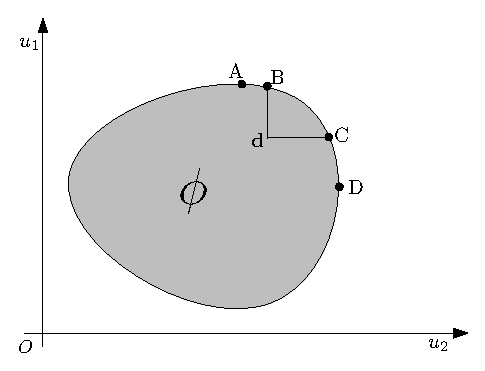
\includegraphics[width = \textwidth]{bargain_basic_concept} 
    \caption{议价概念示意图} 
    \label{fig:chap_bargain:bargain_basic_concept} 
  \end{minipage}%
\end{figure}


\section{资源分配博弈模型}
在一个资源受限的系统中,存在有~$n$~个用户。
他们以合作的方式或“议价”的方式来分配网络所提供的资源,例如带宽。
每一个用户都有自己的效用函数~$U_i(b_i)$~。
效用函数由它当前分配到的带宽~$b_i$~、期望申请到的带宽~$B_i^{req}$~和一个最低效用~$U_i(b_{0i})$~决定。
最低效用也被定义为“分歧点”;用户为了防止最终没能达成合作协议时预先确定会得到的效用。
令~$\phi = \{ \mathbf{U} \} \subset R^n$~为效用的集合,其中,~$\mathbf{U} =(U_1(b_1), \ldots, U_n(b_n))$~。令~$\mathbf{d} = (d_1, \ldots, d_n)$~是用户的分歧点,其中,~$d_i = U_i(b_{0i})$~。
所以,我们可将此博弈问题定义为 ~$(\mathbf{\phi,d})$~。
接下来我们来描述博弈的细节。

首先是博弈参与者效用的定义。
在前面章节(呼叫接纳控制算法)中,我们曾经定义过服务质量水平。
此处我们延用指数函数归一化形式来定义用户连接的QoS水平,如\eqref{eqn:chap_nash:qos_definition} 所示。
\begin{equation}
QoS = \frac{1- e^{-\rho \frac{b}{B} }}{1-e^{-\rho}}, \rho > 0
\label{eqn:chap_nash:qos_definition}
\end{equation}
其中,$b$ 表示博弈参与者最终分配到的资源。
$B$表示博弈者在提交申请时,希望能够分配到的资源数量。
$\rho$表示业务的特征值。

因为QoS的大小与$\rho \frac{b}{B}$紧密相关,
且\eqref{eqn:chap_nash:qos_definition}是单调增函数,
所以我们定义如下效用的简化计算公式,如 \eqref{eqn:chap_nash:utility_definition}所示。
\begin{align}
    U_i(b_i) = \rho_i \frac{b_i}{B_i^{req}}
    \label{eqn:chap_nash:utility_definition}
\end{align}
其中,下标$i$是指系统中的第$i$个博弈参与者。
因为$b_i\ge 0$,且$B_i^{req}$和$\rho$都大于零,所以$U_i(b_i)\ge0$。
另一方面,由于系统的资源是有限的,所以要求$\sum_i^n \le B_{total}$
其中,$B_{total}$是系统所能提供的资源数量。
对于分歧点,我们假设每个博弈参与者有一个最低资源要求~$B_i^{\min}$~,
则~$d_i = \rho_i \frac{B_i^{\min}}{B_i}$~。同时也要求~$b_i > B_i^{\min}$~。

\section{非对称纳什议价解}
\begin{figure}[!tb] 
    \centering
   \begin{minipage}[t]{0.5\linewidth} 
    \centering 
    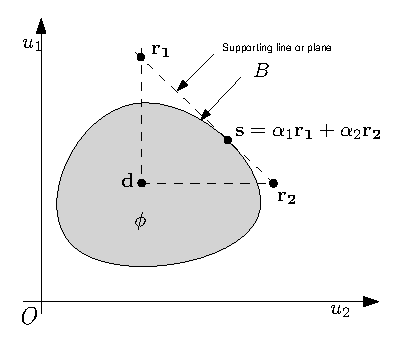
\includegraphics[width = \textwidth]{chap_nash_2_dim_nash_bargain.eps} 
    \caption{两用户议价解示意图} 
    \label{fig:chap_bargain:2_dim_nash_bargain} 
  \end{minipage}%
\end{figure}

我们先定义议价博弈的数学形式,然后再分析它的解的情况。
博弈的解从数学上的表示,其实是一个映射函数,即,$F: \mathbf{\phi} \rightarrow R^n$,
记作$F(\phi, \mathbf{d})$。

符合帕累托最优的博弈解在效用集合的一部分边界上,这部分边界记作$B$。
$\mathbf{s}$表示这部分边界上的点,用如下 \eqref{eqn:chap_nash:points_bargain}表示。
\begin{align}
 \mathbf{s} = \sum_{i=1}^n \alpha_i \mathbf{r}_i
    \label{eqn:chap_nash:points_bargain}
\end{align}
其中,$\alpha_i$表示议价能力,且满足$\sum_{i=1}^n \alpha_i = 1$。
$\mathbf{r}_i, i= 1,\dots,n$是$n$维空间中一个点。$\mathbf{s} = \alpha_i \mathbf{r}_i$可理解为多维空间的一个超平面,且与集合$\phi$只有一个交点,此平面也称为支撑平面(supporting plane),记为 $S$。
如果以分歧点为起始点,画出$n$条与空间坐标轴平行的线,那么这些平行线与平面$S$的交点就是$\mathbf{r}_i, i= 1,\dots,n$。
所有满足上述条件的点的集合记作$B$,博弈论中也称之为可行集。
例如在二维情况下,这个超平面退化为是一条支撑线(supporting line),而这些点$\mathbf{r}_i, i= 1,2$就是与过分歧点与横轴平行的线、与纵轴平行的线的交点,
如\figref{fig:chap_bargain:2_dim_nash_bargain}所示。
综上所述,议价博弈的符合帕累托最优的解可以写为\eqref{eqn:chap_nash:game_solution},
\begin{align}
    F(\mathbf{\phi},\mathbf{d}) = \left\{ \mathbf{s} \in \mathbf{B} \big \vert \mathbf{s} = \sum_{i=1}^n \alpha_i \mathbf{r}_i \right\}
    \label{eqn:chap_nash:game_solution}
\end{align}
同时,点$\mathbf{s}$也是集合$\phi$边界上的点。

因为一般符合帕累托最优的议价解不止一个,经济学家纳什提出了如果满足一些条件,
那么就可以确定一个唯一合理的解\cite{Nash_1950}。

\subsection{纳什公理化议价博弈理论}
首先假定在一个博弈过程中存在两个参与者。
每个博弈的参与者追求使自己的效用最大化。
我们把它们分别记为~$u_1$~和~$u_2$~。
记号~$\phi$~表示效用向量~$\mathbf{u}=(u_1, u_2)$~的非空紧凸集合(Closed and bounded)。
并且,双方附加一个条件:如果博弈双方不能达成一个有约束力的协议的话,
那么,双方将会得到效用~$\mathbf{b}=(d1, d2)$~。
效用向量~$\mathbf{d}$~也被叫作“分歧点”(disagreement points)。
纳什议价博弈模型的解是这样一个函数~$f$~,该函数可以将集合~$\phi$~映射到解集上。
纳什还提出以下公理:

\begin{itemize}
\item 公理一:个体理性(Individual Rationality) 
    对于用户~$i$~而言, ~$u_i^* \ge d_i$~
\item 公理二:可行性(Feasibility),解满足关系式~$\mathbf{u}^* \in \phi$~
\item 公理三:弱帕累托最优性质(Weak Pareto Optimality)\\
如果~$\mathbf{u} \in \phi$~,而且~$\mathbf{u} \ge \mathbf{u}^*$~,那么可以推导得到 ~$\mathbf{u} = \mathbf{u}^*$~
\item 公理四:对称性(Symmetry),\\
如果~$d1=d2$~ 并且如果~$(u_1, u_2) \in \phi \Rightarrow (u_2, u_1) $~, 一定有 ~$u_1^*= u_2^*$~。
\item 公理五:线性变换无关( Independence of Linear Transformations)\\ 
如果~$\forall (a_1, a_2, b_1, b_2) \in R$~,如果我们定义函数~$g$~是将所有向量~$(u1, u2)$~映射到~$(u1', u2')$~的线性变换函数,例如~$u_i^\prime=a_iu_i+ b_i (i =1,2)$~,于是我们有 ~$f[g(\phi), g(d)]=g[f(\phi , d)]$~。
\item 公理六:无关选择的无关性(Independence of Irrelevant Alternatives) \\
如果集合~$\psi \subset \phi$~ ,
并且~$f(\phi,d) \in \psi$~,那么可得 ~$f(\psi,d) = f(\phi,d)$~ 。
\end{itemize}
其中,公理一、公理二和公理三定义了议价解集合~$B$~。
纳什议价解(Nash Bargaining Solution,NBS)也在议价解集合中。
公理三保证了集体理性,在议价可能集内不再存在议价双方好于议价角的效用向量。
公理四、公理五和公理六称为公平性公理。
公理四描述了如果用户有相同的“分歧点”(disagreement points)和效用函数,那么它们的效用一定相同。
对称博弈中博弈双方有完全相同的策略可能性及相同的议价能力。
公理五表明如果效用变换函数如果是线性的,那么最终议价解是不变的。
公理六表明如果在一个集合的议价解在一个小的子集内找到,这个子集的解也就是这个集合的解。
如果逐步从原来的可行集中排除一些无关选择,并不改变最终的议价解。
这在议价的过程中可以解释为博弈双方可以自愿地相互让步。
而它的数学含义是,议价仅仅依赖于$\mathbf{u}^*$领域可行集右上边界的形状。

如果满足以上公理的情况下,
可以证明纳什议价的唯一解便是使纳什积最大化的效用向量\cite{Nash_1950},即
\begin{align}
\mathbf{u}^* = \arg \max \prod_i^n (u_i-d_i)
\label{eqn:chap_nash:nash_product}
\end{align}


由博弈的定义可看出,我们博弈模型首先可以满足公理一、二、四。
因为公理三、五和六所描述的内容,从数学上来首先要求效用集合是凸集。
所以,我们下面证明在我们定义资源分配的效用向量集合$\mathbf{\phi}$是凸集(convex set)。

定理:如果效用向量集合$\mathbf{\phi}$中的元素如\eqref{eqn:chap_nash:utility_definition}所定义,那么它是一个凸集。

证明:我们知道,如果一个集合$\mathbf{\phi}$是凸集,
那么对这个集合中的任意两个元素,$\mathbf{x}$和$\mathbf{y}$,以及一个任意的数$\theta$, $0\le \theta\le 1$来说,凸组合$\mathbf{z}=\theta \mathbf{x} + (1-\theta) \mathbf{y}$所构成的元素也属于集合$\mathbf{\phi}$。

我们用大写记号$\mathbf{X}$ 和$\mathbf{Y}$表示博弈效用集合中的任意两个元素,则有
\begin{align*}
    \mathbf{X} &=\left( (U(b_1), U(b_2), \ldots, U(b_n) \right)
    = \left( \rho_1 \frac{b_1}{B_1^{req}},\rho_2 \frac{b_2}{B_2^{req}},\ldots, \rho_n \frac{b_n}{B_n^{req}} \right) \in \mathbf{\phi} \\
    \mathbf{Y} &=\left( (U(b_1^\prime), U(b_2^\prime), \ldots, U(b_n\prime) \right)
    = \left( \rho_1 \frac{b_1^\prime}{B_1^{req}},\rho_2 \frac{b_2^\prime}{B_2^{req}},\ldots, \rho_n \frac{b_n^\prime}{B_n^{req}} \right) \in \mathbf{\phi} 
    %\label{eqn:chap_nash:two_elements}
\end{align*}
其中,$(b_1, b_2, \ldots, b_n)$和 $(b_1^\prime, b_2^\prime, \ldots, b_n^\prime)$是分配的资源数量,且满足$b_i \ge 0$ ,$b_i^\prime \ge 0$, $i = 1, \ldots, n$。
则有,
\begin{align*}
    U(b_i) &= \rho_i \frac{b_i}{B_i^{req}} \Rightarrow b_i = \frac{U(b_i)B_i^{req}}{\rho_i} \\
    U(b_i^\prime) & \rho_i \frac{b_i^\prime} {B_i^{req}} \Rightarrow b_i^\prime = \frac{U(b_i^\prime) B_i^{req}}{\rho_i}
\end{align*}
由于资源是受限的,所以还要满足下面的不等式关系
\begin{align*}
    \sum_{i=1}^n b_i \le B_{total} \Rightarrow \sum_{i=1}^n \frac{U(b_i)B_i^{req}}{\rho_i} \le B_{total}\\
    \sum_{i=1}^n b_i^\prime \le B_{total}\Rightarrow \sum_{i=1}^n \frac{U(b_i^\prime)B_i^{req}}{\rho_i} \le B_{total}
    %\label{eqn:chap_nash:in-equation}
\end{align*}
接下来对于凸组合$\mathbf{Z}$ 则有,
\begin{align*}
    \mathbf{Z} = \left( \theta U(b_1) + (1-\theta) U(b_1^\prime),   \theta U(b_2) + (1-\theta) U(b_2^\prime), \ldots,  \theta U(b_n) + (1-\theta) U(b_n^\prime) \right)
\end{align*}
因此,如果$\mathbf{Z}$属于集合$\mathbf{\phi}$,那么一定会存在等价命题,即,
\begin{align}
    \sum_{i=1}^{n} \frac{ \theta U(b_i) + (1-\theta) U(b_i^\prime)}{\rho_i}  \le B_{total}
    \label{eqn:chap_nash:proof_z_in_s}
\end{align}
为了证明\eqref{eqn:chap_nash:proof_z_in_s} 成立,则让
\begin{align*}
    &\sum_{i=1}^{n} \frac{ \theta U(b_i) + (1-\theta) U(b_i^\prime)}{\rho_i} - B_{total} \\
    &= \theta \sum_{i=1}^n \frac{U(b_i)B_i^{req}}{\rho_i} + (1-\theta) \frac{U(b_i^\prime)B_i^{req}}{\rho_i} -B_{total} \\
    &\le \theta B_{total} + (1-\theta)B_{total} - B_{total}\\
    & \le 0
\end{align*}
所以,
凸组合$\mathbf{Z}$也是属于集合$\mathbf{\phi}$的,集合$\mathbf{\phi}$是凸集。证明完毕。

同时,我们还注意到,由于$b_i$的定义域是$[0,B_i^{req}]$,且$B_i^{req}$不会是零,所以集合
$\mathbf{\phi}$也是有界且是闭的(bounded and close)。又因最终的纳什议价解是在凸集的边界上,我们的博弈模型也是满足其它公理的描述。

对于资源的分配而言,由于假设博弈参与者的业务不同,所以,博弈参与者对于资源需求程度也就有所不同。
在议价博弈中,还可以假设博弈的参与者在博弈过程中的议价能力不同。这样的假设会使得对称性公理不能满足。
一般我们把不满足对称性公理的议价解称之为非对称纳什议价解(Asymmetric Nash Bargaining Solution)
或称作一般纳什议价解(Generalized  Nash  Solution)。
经济学家已经证明,不满足对称公理的非对称纳什议价解仍可以唯一地确定下来\cite{Osborne_Rubinstein_1994}。
最终的解也同样可以通过使纳什积最大化来求得。

综上所述,我们可以将求解纳什议价解的过程,
转化为求解纳什积的最大化问题,如\eqref{eqn:chap_nash:maximum_problem} 所定义。
\begin{align}
    \mathbf{b}^* &= \arg \max G(\mathbf{U}, \mathbf{d}) = \prod_{i=1}^n (U(b_i) - d_i)^{\alpha_i} = \prod_{i=1}^{n} \left(\rho_i \frac{b_i}{B_i^{req}} - \rho_i \frac{B_i^{\min}}{B_i^{req}} \right)^{\alpha_i} \notag\\
    & s.t. \quad \sum_i^n b_i \le B_{total} 
    \label{eqn:chap_nash:maximum_problem}
\end{align}


为了简化求解的过程,我们对$G(\mathbf{U}, \mathbf{d})$两边取自然对数,则有
\begin{align}
    \ln G(\mathbf{U}, \mathbf{d}) &= \sum_{i=1}^{n} \ln \left(\rho_i \frac{b_i}{B_i^{req}} - \rho_i \frac{B_i^{\min}}{B_i^{req}} \right)^{\alpha_i} \notag \notag\\
    &= \sum_{i=1}^n \left[ \alpha_i \ln \left( \frac{\rho_i}{B_i^{req}} \right) + \alpha_i \ln \left( b_i - B_i^{\min} \right) \right] \notag\\
    &= \sum_{i=1}^n \alpha_i \ln \left( \frac{\rho_i}{B_i^{req}} \right) + \sum_{i=1}^n  \alpha_i \ln \left(b_i - B_i^{\min} \right) 
    \label{eqn:chap_nash:ln_format}
\end{align}
因为$\rho_i, \alpha_i, B_i^{req}$均是已知的系数,所以,\eqref{eqn:chap_nash:ln_format} 第一项为常数。
则,上面优化问题可改写等价的问题为
\begin{align}
    \mathbf{b}^* &= \arg \max Q(\mathbf{U}, \mathbf{d}) = \sum_{i=1}^n  \alpha_i \ln \left( b_i - B_i^{\min} \right) \notag\\
    & s.t. \quad \sum_i^n b_i \le B_{total} 
\end{align}

下面我们通过拉格朗日乘数法来求解 $\mathbf{b}^*$。
整个过程分为两步,第一步求可能的极值点,第二步判断是否是极大值。

为了找到函数$Q(\mathbf{U}, \mathbf{d})$在条件$\sum_i^n b_i \le B_{total}$下的可能极值点,
先构造函数
\begin{align*}
    F(\mathbf{U}, \mathbf{d}) =  \sum_{i=1}^n  \alpha_i \ln \left(b_i - B_i^{\min} \right)
    + \lambda(\sum_i^n b_i - B_{total} ) 
\end{align*}
其中,$\lambda$为拉格朗日乘子,然后对每一个$b_i, i=1,\dots,n$求一阶偏导数,
并使之为零,然后约束条件联立起来:
\begin{align}   
    \begin{cases}
        \displaystyle\frac{\alpha_i}{b_i - B_i^{\min}} + \lambda = 0, i=1,\dots, n  \\
        \displaystyle \sum_{i=1}^n b_i - B_{total} = 0
    \end{cases}
\end{align}
则有,
\begin{align*}
    b_i &= B_i^{\min} - \frac{\alpha_i}{\lambda} \\
    \Rightarrow & \sum_{i=1}^n \left[ B_i^{\min} - \frac{\alpha_i}{\lambda} \right] = B_{total} \\
    \Rightarrow & \sum_{i=1}^n B_i^{\min} - \frac{1}{\lambda} \sum_{i=1}^n \alpha_i = B_{total}
\end{align*}
又因$\alpha_i$定义知,
\begin{align*}
    \sum_{i=1}^n \alpha_i = 1
\end{align*}
则可以解出 $\lambda$,
\begin{align*}
    \lambda = \frac{1}{(\sum_{i=1}^n B_i^{\min} )  -B_{total} }
\end{align*}
最后解出$b_i$,
\begin{align}
    b_i = B_i^{\min} + \alpha_i \left( B_{total} - \sum_{i=1}^n B_i^{\min}  \right)
    \label{eqn:chap_nash:res_allocation}
\end{align}
第一步完成,说明此优化问题有唯一驻点。

第二步,为了判断是否是极值点,我们对$F(\mathbf{b},\mathbf{d})$求两阶偏导数,得其海赛矩阵
\begin{align*}
    \nabla ^2 F &= \left[
    \begin{array}{cccc}
        \frac{\partial ^2F}{\partial b_{1} \partial b_1} & \frac{\partial ^2F}{\partial b_{1} \partial b_2} & \cdots &  \frac{\partial ^2F}{\partial b_{1} \partial b_n}\\
        \frac{\partial ^2F}{\partial b_{2} \partial b_1} & \frac{\partial ^2F}{\partial b_{2} \partial b_2} & \cdots &  \frac{\partial ^2F}{\partial b_{2} \partial b_n}\\
         & \cdots \cdots & & \\
        \frac{\partial ^2F}{\partial b_{n} \partial b_1} & \frac{\partial ^2F}{\partial b_{n} \partial b_2} & \cdots &  \frac{\partial ^2F}{\partial b_{n} \partial b_n}
    \end{array} 
    \right] \\
    & = \left[
    \begin{array}{cccc}
        -\frac{\alpha_1}{(b_1-B_1^{\min})^2} & 0 & \cdots & 0\\
        0& -\frac{\alpha_1}{(b_2-B_2^{\min})^2} &\cdots& 0\\
        &\cdots\cdots&&\\
        0& 0 &\cdots & -\frac{\alpha_1}{(b_n-B_n^{\min})^2}\\
    \end{array}
    \right]
\end{align*}
显然此矩阵是一个对角阵。
又因为$\alpha_i>0$,$b_i > B_i^{\min}$,则$-\frac{\alpha_1}{(b_i-B_i^{\min})^2}<0$。
所以$\nabla ^2 F$是负定矩阵。
则使纳什积$G(\mathbf{U},\mathbf{d})$最大的解,即,
\begin{align}
    \mathbf{b}^* = b_i^* = B_i^{\min} + \alpha_i \left( B_{total} - \sum_{i=1}^n B_i^{\min}  \right)
    \label{eqn:chap_nash:nbs}
\end{align}

\section{议价能力}
由\eqref{eqn:chap_nash:nbs}知,
%纳什议价解与资源比例分配算法的结果十分类似。
%在比例分配算法中权重与纳什议价解中的议价能力起到的作用是相同的。
议价能力对用户的QoS的影响十分重要。
如 \figref{fig:chap_nash:two_users_nbs_qos}所示,我们以两用户为例,
对人为设定不同议价能力进行分析。
\footnote{用户$1$与用户$2$的参数设置如下:假设$B_1^{\min}=64Kbps, B_2^{\min}=96Kbps$,$B_1^{req}=256Kbps, B_2^{req}=384Kbps$,$\rho_1=4, \rho_2=5$}
图中用户$1$的议价能力被标记为$\alpha_1$;
用户$2$的议价能力为$1-\alpha_1$。
很明显,随着用户$1$的议价能力提高,用户$1$对资源的竞争力也逐步增强,QoS的值也增大。
相应地,用户$2$的QoS趋势则随着议价能力的下降而下降。
同时,从图中还可以看到,如果系统资源的总量增大,两用户的QoS都会有所改善。
\begin{figure}[!tb] 
    \centering 
    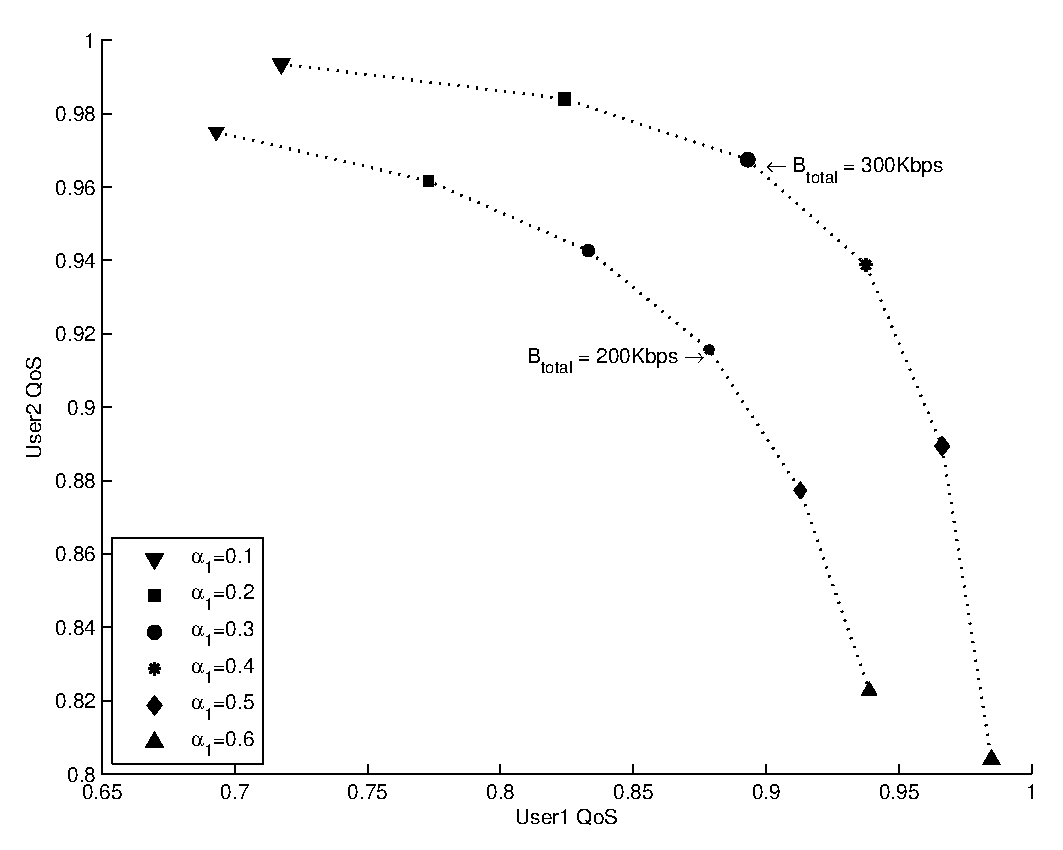
\includegraphics[width = 0.5\textwidth]{chap_nash_two_users_nbs_qos.eps} 
    \caption{两用户议价能力示意图}
    \label{fig:chap_nash:two_users_nbs_qos} 
\end{figure}
那么,如何确定一个用户的议价能力是议价博弈中的一个核心问题。
在我们提出的QoS水平的度量的\eqref{eqn:chap_nash:qos_definition}中,$\rho$被认为是一个描述用户应用特征的一个参数。
从前一章中实验中可以看出,如果$\rho$的值越小,那么它对资源的需求越敏感。相反,$\rho$越大,对资源需求越迟钝。
因此,我们可对应地认为,特征值$\rho$也可以是对竞争能力的一个体现。
则对于某一个用户$i$,他的竞争能力$\alpha_i$可以定义为如下\eqref{eqn:chap_nash:bargaining_power_definition}。
\begin{align}
    \alpha_i = \frac{\frac{1}{\rho_i}}{\sum_{k=1}^n \frac{1}{\rho_k} }
    \label{eqn:chap_nash:bargaining_power_definition}
\end{align}
\section{仿真实验与分析}

\section{小结}
本章我们提出了一个基于纳什议价博弈的资源分配新算法。
首先,我们简单介绍了议价博弈中的基本概念。
然后我们提出了一个新的资源分配议价博弈模型,其中包括用户的效用定义,用户的分歧点设置等。
通过对模型的理论分析,可知我们的模型满足纳什议价公理所提出的约束。
而且,讨论了用户议价能力对分配结果的影响,进而提出以用户应用特征参数值为基础的议价能力的具体定义。
最后结合仿真实验,对所提出的算法进行了验证。
结果表明,所提出的算法,可以有效地且公平地解决用户资源竞争的问题。
新算法在保证系统资源利用的同时,也平衡了各个用户之间的利益。


\cite{yanzw_1}\cite{yanzw_2}
